\documentclass[
11pt, % The default document font size, options: 10pt, 11pt, 12pt
%codirector, % Uncomment to add a codirector to the title page
]{charter} 


% El títulos de la memoria, se usa en la carátula y se puede usar el cualquier lugar del documento con el comando \ttitle
\titulo{Diseño e implementación de motor de afinidad para personalización comercial B2B en consumo masivo} 

% Nombre del posgrado, se usa en la carátula y se puede usar el cualquier lugar del documento con el comando \degreename
\posgrado{Carrera de Especialización en Inteligencia Artificial}

% Tu nombre, se puede usar el cualquier lugar del documento con el comando \authorname
\autor{Lic. Abril Noguera}

% El nombre del director y co-director, se puede usar el cualquier lugar del documento con el comando \supname y \cosupname y \pertesupname y \pertecosupname
\director{Ing. Juan Pablo Rodríguez Varela}
\pertenenciaDirector{ITBA} 
\codirector{} % para que aparezca en la portada se debe descomentar la opción codirector en los parámetros de documentclass
\pertenenciaCoDirector{FIUBA}

% Nombre del cliente, quien va a aprobar los resultados del proyecto, se puede usar con el comando \clientename y \empclientename
\cliente{MSc. Lautaro Gonzalez}
\empresaCliente{Empresa Líder de Consumo Masivo}
 
\fechaINICIO{01 de mayo de 2025}		%Fecha de inicio de la cursada de GdP \fechaInicioName
\fechaFINALPlan{17 de junio de 2025} 	%Fecha de final de cursada de GdP
\fechaFINALTrabajo{19 de diciembre de 2025}	%Fecha de defensa pública del trabajo final

% Agrego paquetes
\usepackage{pgfgantt}
\usepackage{datetime2}
\usepackage{xcolor}

\begin{document}

\maketitle
\thispagestyle{empty}
\pagebreak


\thispagestyle{empty}
{\setlength{\parskip}{0pt}
\tableofcontents{}
}
\pagebreak


\section*{Registros de cambios}
\label{sec:registro}


\begin{table}[ht]
\label{tab:registro}
\centering
\begin{tabularx}{\linewidth}{@{}|c|X|c|@{}}
\hline
\rowcolor[HTML]{C0C0C0} 
Revisión & \multicolumn{1}{c|}{\cellcolor[HTML]{C0C0C0}Detalles de los cambios realizados} & Fecha      \\ \hline
0      & Creación del documento                                 &\fechaInicioName \\ \hline
1      & Se completa hasta el punto 5 inclusive                & 13 de mayo de 2025 \\ \hline
2      & Se completa hasta el punto 9 inclusive                 & 20 de mayo de 2025 \\ \hline
%3      & Se completa hasta el punto 12 inclusive                & {día} de {mes} de 202X \\ \hline
%4      & Se completa el plan	                                 & {día} de {mes} de 202X \\ \hline

% Si hay más correcciones pasada la versión 4 también se deben especificar acá

\end{tabularx}
\end{table}

\pagebreak

\section*{Acta de constitución del proyecto}
\label{sec:acta}

\begin{flushright}
Buenos Aires, \fechaInicioName
\end{flushright}

\vspace{2cm}

%Presupuesto: Sueldo (Hora Hombre * 600hs) + Clusters + Compu = $ 13.500.000

Por medio de la presente se acuerda con la \authorname\hspace{1px} que su Trabajo Final de la \degreename\hspace{1px} se titulará ``\ttitle'' y consistirá en el desarrollo e integración de un sistema de recomendación que estime el interés potencial de cada cliente por los productos del portafolio de la empresa, a partir de señales de comportamiento en su canal digital de ventas. El trabajo tendrá un presupuesto preliminar estimado de 600 horas y un costo estimado de \$ 13.500.000, con fecha de inicio el \fechaInicioName\hspace{1px} y fecha de presentación pública el \fechaFinalName.

Se adjunta a esta acta la planificación inicial.

\vfill

% Esta parte se construye sola con la información que hayan cargado en el preámbulo del documento y no debe modificarla
\begin{table}[ht]
\centering
\begin{tabular}{ccc}
\begin{tabular}[c]{@{}c@{}}Dr. Ing. Ariel Lutenberg \\ Director posgrado FIUBA\end{tabular} & \hspace{2cm} & \begin{tabular}[c]{@{}c@{}}\clientename \\ \empclientename \end{tabular} \vspace{2.5cm} \\ 
\multicolumn{3}{c}{\begin{tabular}[c]{@{}c@{}} \supname \\ Director del Trabajo Final\end{tabular}} \vspace{2.5cm} \\
\end{tabular}
\end{table}




\section{1. Descripción técnica-conceptual del proyecto a realizar}
\label{sec:descripcion}

\subsection{Definición del Problema}

En el sector de consumo masivo, especialmente en modelos de negocio \textit{Business-to-Business (B2B)}, estimar el interés potencial entre clientes y productos desempeña un papel crucial en la optimización de estrategias comerciales.  Esta predicción se utiliza para priorizar qué productos sugerir a cada punto de venta en cada ciclo comercial, permitiendo adaptar las recomendaciones a las preferencias y comportamientos reales de cada cliente. En lugar de ofrecer el mismo conjunto de productos a todos los clientes o basarse únicamente en el historial de compra, contar con una calificación de afinidad posibilita ordenar el portafolio según relevancia, potenciar la venta cruzada y mejorar la eficiencia en el uso del canal digital. Además, brinda al equipo comercial una herramienta concreta para planificar visitas, personalizar ofertas y detectar oportunidades antes no visibles, especialmente en productos nuevos o categorías estratégicas.

La naturaleza del negocio B2B trae más complejidad. A diferencia de los consumidores finales, cuyos patrones de compra suelen ser más regulares y predecibles, los minoristas ajustan sus pedidos en función de variables como la estacionalidad, las promociones comerciales y el comportamiento fluctuante de sus propios clientes. Esta variabilidad se acentúa cuando analizamos la marcada diversidad entre los distintos puntos de venta: desde pequeños kioscos urbanos con espacio limitado para exhibición hasta grandes supermercados con capacidad para gestionar amplios surtidos. Cada uno presenta necesidades y capacidades logísticas radicalmente diferentes.

Además, la constante rotación e incorporación de nuevos productos en el portafolio genera un escenario de permanente adaptación. En la práctica se observa que aproximadamente el 12\% del catálogo se renueva anualmente. Este desafío es conocido como "\textit{cold start}", la dificultad para recomendar productos sin historial transaccional. Este problema se vuelve aún más desafiante porque, incluso entre los productos que ya tienen historial de ventas, muchos presentan compras muy esporádicas o aisladas. Esto genera un conjunto de datos con poca información por producto, lo que dificulta que los modelos tradicionales puedan aprender patrones consistentes para hacer buenas recomendaciones.

El ecosistema B2B presenta particularidades que exigen soluciones a medida. Estas deben ir más allá de los enfoques tradicionales de recomendación para incorporar, además de datos transaccionales históricos, información contextual sobre los puntos de venta, señales de comportamiento digital e inteligencia de negocio que permitan capturar las particularidades de cada relación comercial. El desarrollo de este tipo de sistemas permite calcular un \textit{score} de afinidad entre cada cliente y cada producto del portafolio. Esto refleja qué tan relevante podría ser ese ítem para ese punto de venta en un momento determinado. Estas puntuaciones pueden luego ser ordenadas para generar \textit{rankings} personalizados que sirvan como insumo para la toma de decisiones comerciales y habilita una estrategia más proactiva y adaptada al comportamiento real de cada cliente.

\subsection{Descripción Funcional}

La solución se organiza en distintos módulos que trabajan de manera integrada para calcular y actualizar, de forma periódica, un nivel de afinidad entre cada cliente y cada producto. El sistema opera de forma cíclica y está compuesto por cinco bloques funcionales que reflejan las etapas clave del proceso. En la figura \ref{fig:diagBloques} se presenta el diagrama en bloques del sistema. 

\begin{figure}[htpb]
\centering 
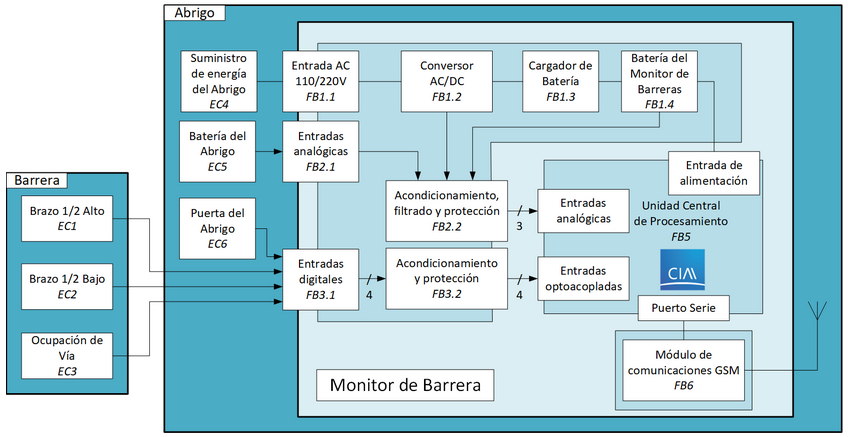
\includegraphics[width=.85\textwidth]{./Figuras/diagBloques.png}
\caption{Diagrama en bloques del sistema.}
\label{fig:diagBloques}
\end{figure}

En primer lugar, se realiza la ingesta y consolidación de la información necesaria para alimentar el modelo. El sistema combina distintas fuentes internas con el objetivo de comprender en profundidad las preferencias de cada punto de venta. Por una parte, se analiza el historial de compras para identificar los productos que han resultado más relevantes según el tipo de negocio. Por otra, se incorpora el registro de interacciones digitales, como búsquedas, visualizaciones y agregados al carrito que no derivaron en una compra. Esta información se completa con características del cliente, como la ubicación, el tamaño del establecimiento y el perfil del consumidor final, junto con atributos del producto, como la categoría, la marca y su posición dentro del portafolio. El objetivo de esta etapa es construir una base robusta que permita representar de manera integral la relación entre clientes y productos.

A continuación, los datos procesados se convierten en variables que resumen el comportamiento del cliente frente a cada producto. Estas variables incluyen la frecuencia y la recencia de las interacciones, la variedad de categorías exploradas y la intensidad de actividad en distintos períodos. También se incorporan indicadores contextuales, como la popularidad del producto en grupos de clientes similares o el nivel de exposición previa. Este conjunto de variables constituye la entrada del modelo que calcula el valor de afinidad entre cada cliente y cada producto.

El valor estimado representa una medida continua que refleja la relevancia potencial de un producto para un punto de venta específico. Esta puntuación permite ordenar los productos según su grado de interés relativo y se actualiza de forma periódica para adaptarse a los cambios en el comportamiento comercial. El modelo utilizado será seleccionado en función de su desempeño, comparando diferentes alternativas con base en las métricas definidas.

Una vez calculadas las puntuaciones, se evalúa la calidad de las recomendaciones a través de métricas específicas del ámbito de los sistemas de recomendación. Entre las más relevantes se encuentran el \textit{recall} en el top K, la cobertura del portafolio, la diversidad de las sugerencias generadas y la precisión media promedio. Estas métricas permiten monitorear el desempeño general del sistema y detectar oportunidades de mejora tanto a nivel global como por segmento de cliente.

Finalmente, los resultados se integran en los procesos comerciales existentes mediante listas priorizadas de productos para cada cliente. Estas recomendaciones pueden ser visualizadas en la aplicación de ventas o utilizadas por el equipo comercial como herramienta de planificación. De esta forma, el sistema aporta valor concreto al negocio al facilitar sugerencias más relevantes, alineadas con el comportamiento observado y consistentes con los objetivos comerciales de la compañía.

\section{2. Identificación y análisis de los interesados}
\label{sec:interesados}

El proyecto involucra a distintos actores relevantes en su desarrollo, validación y futura aplicación.  El cliente, quien se desempeña como Director del equipo de Data en la \empclientename, es el principal impulsor de la iniciativa y sponsor del proyecto. En particular, se destaca la participación del equipo de Portfolio Strategy como usuario final del sistema, representado por su Product Owner (PO), quien actúa como principal referente funcional articulando entre los requerimientos del negocio y las decisiones técnicas. La responsable directa del desarrollo es la autora de este trabajo, quien llevará adelante el diseño, desarrollo y la implementación de la solución. La siguiente tabla resume estos roles y sus respectivas organizaciones.

\begin{table}[ht]
%\caption{Identificación de los interesados}
%\label{tab:interesados}
\begin{tabularx}{\linewidth}{@{}|l|X|X|l|@{}}
\hline
\rowcolor[HTML]{C0C0C0} 
Rol           & Nombre y Apellido & Organización 	& Puesto 	\\ \hline
% Auspiciante   &                   &              	&        	\\ \hline
Cliente       & \clientename      &\empclientename	& Gerente del Proyecto       	\\ \hline
% Impulsor      &                   &              	&        	\\ \hline
Responsable   & \authorname       & FIUBA        	& Alumno 	\\ \hline
%Colaboradores &                   &              	&        	\\ \hline
Orientador    & \supname	      & \pertesupname 	& Director del Trabajo Final \\ \hline
% Equipo        & miembro1 \newline 
%				miembro2          &              	&        	\\ \hline
% Opositores    &                   &              	&        	\\ \hline
Usuario final &  Lic. Micaela Bassan    & \empclientename	&  Product Owner \\ \hline
\end{tabularx}
\end{table}

\section{3. Propósito del proyecto}
\label{sec:proposito}

El propósito del proyecto es desarrollar un sistema que estime la relevancia potencial de cada producto para cada punto de venta, a partir de información transaccional, comportamientos digitales y atributos contextuales.  Esta estimación permitirá generar listas personalizadas que orienten la planificación comercial y sirvan como insumo para la toma de decisiones. Se busca mejorar la precisión de las sugerencias, ampliar la visibilidad de productos estratégicos y avanzar hacia una gestión más proactiva, escalable y basada en datos, alineada con los objetivos comerciales de la compañía.

\section{4. Alcance del proyecto}
\label{sec:alcance}

El universo sobre el que se desarrollará esta iniciativa corresponde al conjunto de clientes y productos gestionado por el equipo de Portfolio Strategy en Argentina. Este se limita a clientes activos pertenecientes a los canales de Kioscos, Tradicionales y Autoservicios, bajo el régimen \textit{Off Premise}\footnote{Off Premise refiere a puntos de venta donde el producto es adquirido para consumo fuera del establecimiento.}. La cartera de productos considerada se enfoca exclusivamente en bebidas. Quedan excluidos del alcance los clientes de los canales \textit{On Premise}, Supermercados y Mayoristas, dado que presentan dinámicas comerciales significativamente diferentes y representan una fracción menor del total. Tampoco se contempla el negocio de marketplace, debido a sus particularidades operativas y a su peso relativamente reducido dentro del universo analizado.

El desarrollo del proyecto se organiza en una serie de etapas que abarcan desde la exploración inicial del estado del arte hasta la implementación del modelo y su evaluación en entorno real. Estas etapas permiten avanzar de forma iterativa y asegurar la calidad del entregable final, tanto desde el punto de vista técnico como funcional. A continuación, se detallan las principales actividades previstas:

\begin{itemize}
\item Relevamiento de modelos \textit{benchmark} y revisión del estado del arte.
\item Definición de métricas de éxito del proyecto.
\item Desarrollo de un modelo \textit{baseline} como punto de comparación inicial.
\item Formulación de hipótesis orientadoras del enfoque propuesto.
\item Desarrollo del proceso de \textit{feature engineering}.
\item Entrenamiento y validación de modelos.
\item Evaluación de resultados con métricas de recomendación.
\item Construcción del pipeline de implementación.
\item Ejecución de pruebas tipo A/B.
\item Reporte y presentación de resultados.
\item Registro y disponibilización del modelo final en MLflow.
\end{itemize}

Si bien este desarrollo se enmarca en un universo específico de clientes y productos, el enfoque está diseñado de manera modular, con el objetivo de facilitar su adaptación a otros segmentos del negocio en caso de resultar exitoso.

\section{5. Supuestos del proyecto}
\label{sec:supuestos}

Para el desarrollo del presente proyecto se supone que: 
\begin{itemize}
	\item Se cuenta con acceso a las fuentes de información necesarias para el desarrollo de la solución. 
        \item No se producirán cambios significativos en los procesos comerciales o en la estructura de los datos durante el período de desarrollo.
	\item Se dispone con los accesos a recursos cloud y software necesarios para el desarrollo de la solución. 
	\item El tiempo asignado para completar el proyecto será suficiente.
        \item Los colaboradores e interesados clave disponen del tiempo para reuniones de validación y toma de decisiones.
\end{itemize}

\section{6. Product Backlog}
\label{sec:backlog}

La siguiente sección presenta el Product Backlog del proyecto, estructurado en torno a cuatro épicas principales que agrupan las funcionalidades clave del desarrollo. Cada épica contiene historias de usuario redactadas de forma concisa, con el objetivo de representar las necesidades del sistema desde la perspectiva de los distintos roles involucrados. Las historias incluyen su prioridad relativa, una estimación en Story Points y una breve descripción del propósito funcional. La asignación de Story Points se basa en una evaluación multidimensional que considera dificultad, complejidad e incertidumbre, redondeando el valor total al número superior más próximo dentro de la secuencia de Fibonacci. Este enfoque busca facilitar la planificación de los sprints y asegurar la trazabilidad entre objetivos, funcionalidades y entregables.

\subsection*{\'Epica 1: \textit{Discovery} y entendimiento del problema}
\begin{itemize}
  \item \textbf{Historia:} Como responsable del proyecto, quiero relevar y documentar las expectativas del cliente para alinear el desarrollo con sus objetivos.\\
  \textbf{Prioridad:} Alta, \textbf{Story Points:} 3, \textbf{Justificación:} D:2, C:1, I:2 $\Rightarrow$ Total: 5

  \item \textbf{Historia:} Como analista, quiero revisar el estado del arte para incorporar enfoques relevantes y detectar oportunidades.\\
  \textbf{Prioridad:} Media, \textbf{Story Points:} 5, \textbf{Justificación:} D:2, C:2, I:3 $\Rightarrow$ Total: 7

  \item \textbf{Historia:} Como responsable del proyecto, quiero definir KPIs y métricas para medir el desempeño de la solución.\\
  \textbf{Prioridad:} Alta, \textbf{Story Points:} 3, \textbf{Justificación:} D:2, C:1, I:2 $\Rightarrow$ Total: 5
\end{itemize}

\subsection*{\'Epica 2: Desarrollo de ingeniería de atributos}
\begin{itemize}
  \item \textbf{Historia:} Como desarrolladora, quiero construir un proceso de extracción, transformación y carga (\textit{ETL}) que asegure calidad y consistencia en los datos.\\
  \textbf{Prioridad:} Alta, \textbf{Story Points:} 5, \textbf{Justificación:} D:3, C:2, I:2 $\Rightarrow$ Total: 7

  \item \textbf{Historia:} Como analista, quiero realizar un análisis exploratorio para entender patrones y relaciones en los datos.\\
  \textbf{Prioridad:} Alta, \textbf{Story Points:} 3, \textbf{Justificación:} D:2, C:2, I:1 $\Rightarrow$ Total: 5

  \item \textbf{Historia:} Como científica de datos, quiero construir variables relevantes para representar el comportamiento de clientes y productos.\\
  \textbf{Prioridad:} Alta, \textbf{Story Points:} 5, \textbf{Justificación:} D:3, C:2, I:2 $\Rightarrow$ Total: 7
\end{itemize}

\subsection*{\'Epica 3: Modelado y Evaluación}
\begin{itemize}
  \item \textbf{Historia:} Como responsable técnica, quiero desarrollar un modelo \textit{baseline} que sirva como comparación inicial.\\
  \textbf{Prioridad:} Media, \textbf{Story Points:} 3, \textbf{Justificación:} D:2, C:2, I:1 $\Rightarrow$ Total: 5

  \item \textbf{Historia:} Como científica de datos, quiero entrenar un modelo más avanzado para estimar afinidad con mayor precisión.\\
  \textbf{Prioridad:} Alta, \textbf{Story Points:} 5, \textbf{Justificación:} D:3, C:2, I:3 $\Rightarrow$ Total: 8

  \item \textbf{Historia:} Como equipo de proyecto, quiero evaluar el rendimiento del modelo con métricas apropiadas.\\
  \textbf{Prioridad:} Alta, \textbf{Story Points:} 3, \textbf{Justificación:} D:2, C:1, I:2 $\Rightarrow$ Total: 5

  \item \textbf{Historia:} Como desarrolladora, quiero registrar el modelo en MLflow para asegurar su trazabilidad.\\
  \textbf{Prioridad:} Media, \textbf{Story Points:} 2, \textbf{Justificación:} D:1, C:1, I:1 $\Rightarrow$ Total: 3
\end{itemize}

\subsection*{\'Epica 4: Implementación}
\begin{itemize}
  \item \textbf{Historia:} Como responsable técnica, quiero preparar un \textit{pipeline} mensual que automatice la generación de \textit{scores}.\\
  \textbf{Prioridad:} Alta, \textbf{Story Points:} 5, \textbf{Justificación:} D:3, C:2, I:3 $\Rightarrow$ Total: 8

  \item \textbf{Historia:} Como analista de negocio, quiero ejecutar una prueba A/B para comparar el impacto del sistema.\\
  \textbf{Prioridad:} Alta, \textbf{Story Points:} 5, \textbf{Justificación:} D:3, C:2, I:3 $\Rightarrow$ Total: 8

  \item \textbf{Historia:} Como responsable del sistema, quiero monitorear el funcionamiento del modelo para asegurar su estabilidad.\\
  \textbf{Prioridad:} Media, \textbf{Story Points:} 3, \textbf{Justificación:} D:2, C:2, I:1 $\Rightarrow$ Total: 5

  \item \textbf{Historia:} Como responsable del proyecto, quiero presentar los resultados a los interesados para facilitar su adopción.\\
  \textbf{Prioridad:} Alta, \textbf{Story Points:} 2, \textbf{Justificación:} D:1, C:1, I:1 $\Rightarrow$ Total: 3
\end{itemize}

\section{7. Criterios de aceptación de historias de usuario}
\label{sec:criteriosAceptacion}

Los criterios de aceptación definen de forma objetiva cuándo una historia de usuario se considera completa y correctamente implementada. Están redactados de manera específica, medible y verificable, con el objetivo de validar que cada funcionalidad cumple con los requerimientos funcionales, técnicos y de presentación.

\textbf{\'Epica 1: \textit{Discovery} y entendimiento del problema}
\begin{itemize}
  \item HU1: Definir expectativas del cliente
  \begin{itemize}
    \item Se entrega un documento con los objetivos y necesidades del cliente validados por el sponsor.
    \item El documento se revisa en una reunión de validación.
  \end{itemize}
  \item HU2: Analizar estado del arte
  \begin{itemize}
    \item Se entrega un informe con mínimo tres enfoques de referencia.
    \item El análisis incluye fortalezas y debilidades por enfoque.
    \item El PO valida la aplicabilidad a este caso.
  \end{itemize}
  \item HU3: Definir métricas
  \begin{itemize}
    \item Se definen al menos tres métricas clave (recall, MAP, cobertura).
    \item Se documenta su forma de cálculo.
    \item Se aprueban en conjunto con el equipo técnico.
  \end{itemize}
\end{itemize}

\textbf{\'Epica 2: Desarrollo de ingenier\'ia de atributos}
\begin{itemize}
  \item HU4: Construir proceso ETL
  \begin{itemize}
    \item El pipeline carga correctamente datos de todas las fuentes requeridas.
    \item El código pasa controles básicos de calidad.
    \item Se valida consistencia con una muestra aleatoria de registros.
  \end{itemize}
  \item HU5: Realizar EDA
  \begin{itemize}
    \item Se entrega notebook con análisis descriptivo de las principales variables.
    \item Se identifican valores faltantes, atípicos y distribuciones.
    \item Los hallazgos se documentan y discuten en revisión técnica.
  \end{itemize}
  \item HU6: Generar atributos
  \begin{itemize}
    \item Se construyen al menos 10 variables relevantes para el modelo.
    \item Se justifica cada atributo en función de comportamiento cliente-producto.
    \item Se validan estadísticas básicas y cobertura para cada \textit{feature}.
  \end{itemize}
\end{itemize}

\textbf{\'Epica 3: Modelado y Evaluación}
\begin{itemize}
  \item HU7: Desarrollar modelo baseline
  \begin{itemize}
    \item Se entrena un modelo sencillo como punto de referencia.
    \item El código está documentado y versionado.
    \item Se reportan las métricas definidas en la sección anterior.
  \end{itemize}
  \item HU8: Desarrollar modelos benchmark
  \begin{itemize}
    \item El modelo final obtiene mejora en al menos 2 métricas frente al baseline.
    \item El pipeline de entrenamiento es reproducible.
    \item Se valida su comportamiento en distintos segmentos de cliente.
  \end{itemize}
  \item HU9: Evaluación completa
  \begin{itemize}
    \item Se presentan los resultados completos por métrica y segmento.
    \item Se identifican debilidades del modelo y posibles mejoras.
    \item Se valida el cumplimiento de los objetivos del proyecto.
  \end{itemize}
  \item HU10: Registro en MLflow
  \begin{itemize}
    \item El modelo se encuentra registrado con nombre, fecha, parámetros y métricas.
    \item Se puede reproducir y reutilizar desde el entorno técnico.
    \item Su versión queda asociada al entregable final.
  \end{itemize}
\end{itemize}

\textbf{\'Epica 4: Implementación}
\begin{itemize}
  \item HU11: Pipeline de producción
  \begin{itemize}
    \item El proceso mensual corre sin errores y genera resultados válidos.
    \item El output se integra al flujo operativo existente.
    \item Se documenta el proceso completo.
  \end{itemize}
  \item HU12: A/B Testing
  \begin{itemize}
    \item Se define correctamente el grupo de control y tratamiento.
    \item Se mide el impacto de forma cuantitativa.
    \item El análisis es presentado con visualizaciones claras.
  \end{itemize}
  \item HU13: Seguimiento de salubridad
  \begin{itemize}
    \item Se implementa un control automático de métricas clave.
    \item Se definen alertas en caso de desviaciones significativas.
    \item El equipo puede monitorear mensualmente los resultados.
  \end{itemize}
  \item HU14: Presentación final
  \begin{itemize}
    \item Se elabora una presentación con objetivos, resultados y próximos pasos.
    \item Se presenta al equipo de datos y al PO.
    \item Se entrega junto con el entregable técnico final.
  \end{itemize}
\end{itemize}

\section{8. Fases de CRISP-DM}

El desarrollo del presente proyecto se estructura siguiendo la metodología CRISP-DM  \textit{(Cross Industry Standard Process for Data Mining)}, ampliamente utilizada en proyectos de ciencia de datos por su enfoque iterativo, modular y orientado al negocio. Esta metodología permite alinear los objetivos técnicos con las necesidades estratégicas, estructurando el trabajo en fases que abarcan desde la comprensión del problema hasta la evaluación del modelo y su eventual implementación. A continuación, se detallan las principales etapas de CRISP-DM aplicadas a este caso.

\begin{enumerate}
\item \textbf{Comprensión del negocio:}
El objetivo del proyecto es desarrollar un sistema que permita estimar la relevancia potencial de cada producto para cada punto de venta, con el fin de generar rankings personalizados que orienten las recomendaciones comerciales. El valor agregado de aplicar inteligencia artificial en este contexto radica en mejorar la precisión de las sugerencias, aumentar la cobertura del portafolio y optimizar la eficiencia del canal digital B2B. Las métricas de éxito incluyen recall@K, cobertura, MAP@K y diversidad de recomendaciones.

\item \textbf{Comprensión de los datos:}
Los datos utilizados provienen de fuentes internas de la empresa e incluyen información transaccional, eventos digitales de la aplicación de ventas (visualizaciones, carritos, búsquedas) y atributos contextuales de productos y puntos de venta. La base de datos abarca clientes activos de los canales Kioscos, Tradicionales y Autoservicios bajo régimen Off Premise, y se enfoca en productos del portafolio de bebidas. Se realizará un análisis exploratorio para evaluar la calidad, consistencia y completitud de los datos.

\item \textbf{Preparación de los datos:}
Esta etapa incluye la construcción de un pipeline de ETL que permita integrar y transformar los datos en una estructura analítica adecuada. Se generarán variables que capturen comportamiento histórico, exposición a productos, patrones de navegación y similitud con otros puntos de venta. La ingeniería de atributos buscará representar de manera compacta la relación cliente-producto con el objetivo de alimentar los modelos de predicción de afinidad.

\item \textbf{Modelado:}
Se abordará un problema de recomendación basado en afinidad, utilizando técnicas de aprendizaje supervisado y de filtrado colaborativo, entre otras. Se explorarán algoritmos como modelos de regresión regularizada, matrices de factorización, y eventualmente modelos de ranking o aprendizaje profundo, dependiendo del rendimiento alcanzado por las alternativas más simples.

\item \textbf{Evaluación del modelo:}
El desempeño de los modelos será evaluado utilizando métricas propias del dominio de sistemas de recomendación, tales como recall@K, MAP@K, cobertura del portafolio sugerido y diversidad. La validación se realizará tanto de forma global como segmentada por tipo de cliente o categoría de producto. Los resultados serán comparados contra un modelo baseline y validados junto al equipo funcional.

\item \textbf{Despliegue del modelo:}
En caso de ser validado, el modelo se integrará al sistema de recomendaciones mensuales de la empresa a través de un pipeline automatizado. Los \textit{scores} generados se disponibilizarán en tablas de resultados que alimentan tanto la aplicación de ventas como las herramientas internas del equipo de Portfolio Strategy. El modelo será registrado y versionado en MLflow para facilitar su mantenimiento y evolución.
\end{enumerate}

\section{9. Desglose del trabajo en tareas}
\label{sec:wbs}

A partir de cada historia de usuario definida en el Product Backlog, se identifican tareas técnicas específicas y medibles. Estas tareas permiten una planificación más precisa del proyecto y constituyen la base para la definición de los sprints y del cronograma general. Las tareas están priorizadas según su impacto funcional y su necesidad para cumplir los criterios de aceptación asociados.

\begin{longtable}{|p{2cm}|p{10cm}|c|c|}
\hline
\rowcolor[HTML]{C0C0C0}
Historia de usuario & Tarea técnica & Estimación & Prioridad \\ \hline
\endfirsthead

\hline
\rowcolor[HTML]{C0C0C0}
Historia de usuario & Tarea técnica & Estimación & Prioridad \\ \hline
\endhead

HU1 & Levantar y documentar requerimientos con el sponsor. & 16 hs & Alta \\ \hline

HU2 & Investigar al menos tres enfoques aplicados a problemas similares & 17 hs & Media \\ \hline

HU3 & Seleccionar métricas relevantes junto al equipo técnico & 12 hs & Alta \\ \hline

HU4 & Diseñar pipeline de ingestión desde cada fuente de datos & 16 hs & Alta \\ \hline
HU4 & Implementar transformación de datos  & 12 h & Alta \\ \hline
HU4 & Testear integridad y consistencia de los datos ingresados & 12 hs & Alta \\ \hline

HU5 & Explorar variables claves: frecuencias, correlaciones & 8 hs & Alta \\ \hline
HU5 & Detectar y tratar valores extremos y nulos & 7 hs & Alta \\ \hline
HU5 & Presentar hallazgos del EDA en una revisión técnica & 6 hs & Media \\ \hline

HU6 & Diseñar \textit{features} & 30 hs & Alta \\ \hline
HU6 & Validar el impacto de los atributos de cold start en modelos previos & 6 hs & Alta \\ \hline
HU6 & Desarrollar embeddings para representar clientes y productos & 7 hs & Alta \\ \hline
HU6 & Aplicar técnicas de reducción de dimensionalidad (PCA/TSNE) & 6 hs & Media \\ \hline
HU6 & Validar robustez de \textit{features} ante cambios temporales & 6 hs & Alta \\ \hline
HU6 & Documentar estructura modular & 5 hs & Media \\ \hline
HU6 & Evaluar cobertura y correlación de atributos construidos & 6 hs & Alta \\ \hline
HU6 & Analizar la importancia de cada \textit{feature} en modelos preliminares & 6 hs & Alta \\ \hline
HU6 & Documentar lógica de construcción de \textit{features} & 5 hs & Media \\ \hline
HU6 & Validar \textit{features} construidas con \textit{feedback} del negocio & 6 hs & Alta \\ \hline

HU7 & Implementar y evaluar modelo baseline (top-n por frecuencia) & 14 hs & Media \\ \hline

HU8 & Implementar y evaluar matriz de factorización con ALS & 20 hs & Alta \\ \hline
HU8 & Implementar y evaluar modelo de regresión regularizada & 20 hs & Alta \\ \hline
HU8 & Implementar y evaluar modelo basado en ranking (LightFM o XGBoostRanker) & 20 hs & Alta \\ \hline
HU8 & Implementar y evaluar modelo basado en autoencoders o deep learning & 20 hs & Alta \\ \hline
HU8 & Implementar validación cruzada estratificada por clúster & 8 hs & Alta \\ \hline
HU8 & Analizar varianza de métricas entre folds & 10 hs & Alta \\ \hline
HU8 & Comparar estabilidad de modelos entre splits temporales & 6 hs & Alta \\ \hline
HU8 & Comparar resultados por segmento de cliente & 8 hs & Alta \\ \hline
HU8 & Ajustar hiperparámetros y seleccionar el mejor modelo & 8 hs & Alta \\ \hline
HU8 & Analizar sensibilidad del modelo ante cambios en features clave & 6 hs & Media \\ \hline
HU8 & Evaluar desempeño de modelos en escenario de cold start & 12 hs & Alta \\ \hline
HU8 & Evaluar escalabilidad y tiempos de inferencia de cada modelo & 6 hs & Media \\ \hline
HU8 & Explicar modelo con SHAP o LIME & 6 hs & Alta \\ \hline
HU8 & Validar benchmark final con líderes de datos & 8 hs & Alta \\ \hline

HU9 & Evaluar desempeño del modelo según KPIs definidos & 8 hs & Alta \\ \hline
HU9 & Analizar resultados por grupo de clientes y tipo de producto & 6 hs & Media \\ \hline
HU9 & Visualizar cobertura y recall de productos sin historial & 6 hs & Alta \\ \hline
HU9 & Incorporar análisis de cold start en el informe final & 4 hs & Alta \\ \hline
HU9 & Validar resultados con usuarios funcionales del negocio & 6 hs & Alta \\ \hline
HU9 & Redactar informe de hallazgos con visualizaciones por métrica & 13 hs & Media \\ \hline
HU9 & Generar visualizaciones de resultados por clúster & 8 hs & Alta \\ \hline
HU9 & Simular escenarios comerciales con el modelo & 8 hs & Alta \\ \hline
HU9 & Documentar supuestos técnicos y restricciones del modelo & 8 hs & Media \\ \hline
HU9 & Crear manual funcional para usuarios comerciales & 8 hs & Alta \\ \hline
HU9 & Diseñar y testear checklist de control de calidad & 8 hs & Media \\ \hline
HU9 & Simular fallos controlados y validar manejo de errores & 6 hs & Media \\ \hline

HU10 & Crear \textit{script} automatizado de validación post-entrenamiento & 8 hs & Alta \\ \hline
HU10 & Diseñar arquitectura a alojar en \textit{MlFlow} & 14 hs & Alta \\ \hline
HU10 & Definir protocolo de replicación y respaldo de resultados & 5 hs & Alta \\ \hline
HU10 & Implementar pruebas de estrés en \textit{pipeline} de predicción & 6 hs & Alta \\ \hline
HU10 & Documentar arquitectura general & 14 hs & Alta \\ \hline

HU11 & Automatizar proceso mensual & 8 hs & Alta \\ \hline
HU11 & Diseñar esquema de versionado y mantenimiento del \textit{pipeline} & 8 hs & Alta \\ \hline
HU11 & Simular escenarios de actualización mensual y \textit{fallback} & 6 hs & Alta \\ \hline

HU12 & Realizar prueba A/B & 12 hs & Alta \\ \hline
HU12 & Presentar resultados de prueba A/B a \textit{stakeholders} comerciales & 6 hs & Alta \\ \hline

HU13 & Desarrollar \textit{dashboard} de métricas de salubridad & 10 hs & Media \\ \hline
HU13 & Documentar tablero de seguimiento de salubridad & 4 hs & Media \\ \hline

HU14 & Preparar presentación final con \textit{feedback} técnico y funcional & 8 hs & Alta \\ \hline
HU14 & Ajustar narrativa y visualizaciones de resultados finales & 8 hs & Alta \\ \hline
HU14 & Validar entregables con dirección de estrategia comercial & 4 hs & Alta \\ \hline
HU14 & Consolidar documentación técnica y funcional final & 8 hs & Alta \\ \hline

\end{longtable}

El presente desglose contempla un total de 579 horas de trabajo. Esta estimación contempla el desarrollo técnico completo del sistema de recomendación, desde la definición del problema hasta la evaluación y entrega de resultados. Se considera adecuada para el alcance y profundidad del proyecto, y compatible con los lineamientos establecidos para trabajos de esta naturaleza.

\section{10. Diagrama de Gantt}
\label{sec:gantt}

\begin{ganttchart}[
    hgrid,
    vgrid,
    time slot format=isodate,
    x unit=0.3cm,
    y unit title=0.3cm,
    y unit chart=0.3cm,
    bar height=0.3,
    bar label font=\scriptsize,
    bar label node/.append style={align=left,text width=9cm},
    group label font=\bfseries\small,
    calendar week text={\currentweek}
]{2025-05-01}{2025-11-30}

\gantttitlecalendar{year, month=name} \\
\ganttgroup[bar/.append style={fill=gray!40}]{HU1}{2025-05-01}{2025-05-07} \\
\ganttbar[bar/.append style={fill=blue!50}]{HU1.1 - Entrevista con sponsor}{2025-05-01}{2025-05-02} \\
\ganttbar[bar/.append style={fill=blue!50}]{HU1.2 - Acta validada PO}{2025-05-05}{2025-05-05} \\
\ganttbar[bar/.append style={fill=blue!50}]{HU1.3 - Iterar feedback cliente}{2025-05-06}{2025-05-07} \\

\ganttgroup[bar/.append style={fill=gray!40}]{HU2}{2025-05-08}{2025-05-14} \\
\ganttbar[bar/.append style={fill=blue!50}]{HU2.1 - Investigar enfoques}{2025-05-08}{2025-05-09} \\
\ganttbar[bar/.append style={fill=blue!50}]{HU2.2 - Informe comparativo}{2025-05-12}{2025-05-13} \\
\ganttbar[bar/.append style={fill=blue!50}]{HU2.3 - Alineación técnica}{2025-05-14}{2025-05-14} \\

\ganttgroup[bar/.append style={fill=gray!40}]{HU3}{2025-05-16}{2025-05-20} \\
\ganttbar[bar/.append style={fill=blue!50}]{HU3.1 - Seleccionar métricas}{2025-05-15}{2025-05-16} \\
\ganttbar[bar/.append style={fill=blue!50}]{HU3.2 - Documentar KPIs}{2025-05-19}{2025-05-20} \\

\ganttgroup[bar/.append style={fill=gray!40}]{HU4}{2025-05-21}{2025-06-03} \\
\ganttbar[bar/.append style={fill=blue!50}]{HU4.1 - Relevar fuentes datos}{2025-05-21}{2025-05-22} \\
\ganttbar[bar/.append style={fill=blue!50}]{HU4.2 - Pipeline ingestión}{2025-05-23}{2025-05-26} \\
\ganttbar[bar/.append style={fill=blue!50}]{HU4.3 - Transformación de datos}{2025-05-27}{2025-05-28} \\
\ganttbar[bar/.append style={fill=blue!50}]{HU4.4 - Control calidad datos}{2025-05-29}{2025-05-30} \\
\ganttbar[bar/.append style={fill=blue!50}]{HU4.5 - Testeo consistencia}{2025-06-02}{2025-06-03} \\

\ganttgroup[bar/.append style={fill=gray!40}]{HU5}{2025-06-04}{2025-06-11} \\
\ganttbar[bar/.append style={fill=blue!50}]{HU5.1 - Explorar variables}{2025-06-04}{2025-06-05} \\
\ganttbar[bar/.append style={fill=blue!50}]{HU5.2 - Tratar outliers/nulos}{2025-06-06}{2025-06-09} \\
\ganttbar[bar/.append style={fill=blue!50}]{HU5.3 - Presentar hallazgos}{2025-06-10}{2025-06-11} \\

\ganttgroup[bar/.append style={fill=gray!40}]{HU6}{2025-06-12}{2025-07-17} \\
\ganttbar[bar/.append style={fill=blue!50}]{HU6.1 - Features transaccionales}{2025-06-12}{2025-06-13} \\
\ganttbar[bar/.append style={fill=blue!50}]{HU6.2 - Features digitales}{2025-06-16}{2025-06-17} \\
\ganttbar[bar/.append style={fill=blue!50}]{HU6.3 - Features contextuales}{2025-06-18}{2025-06-19} \\
\ganttbar[bar/.append style={fill=blue!50}]{HU6.4 - Features por segmento}{2025-06-20}{2025-06-23} \\
\ganttbar[bar/.append style={fill=blue!50}]{HU6.5 - Cold start productos}{2025-06-24}{2025-06-25} \\
\ganttbar[bar/.append style={fill=blue!50}]{HU6.6 - Validar cold start}{2025-06-26}{2025-06-27} \\
\ganttbar[bar/.append style={fill=blue!50}]{HU6.7 - Embeddings clientes/productos}{2025-06-30}{2025-07-01} \\
\ganttbar[bar/.append style={fill=blue!50}]{HU6.8 - Reducción dimensionalidad}{2025-07-02}{2025-07-03} \\
\ganttbar[bar/.append style={fill=blue!50}]{HU6.9 - Validar robustez temporal}{2025-07-04}{2025-07-07} \\
\ganttbar[bar/.append style={fill=blue!50}]{HU6.10 - Modularidad futura}{2025-07-08}{2025-07-08} \\
\ganttbar[bar/.append style={fill=blue!50}]{HU6.11 - Cobertura y correlación}{2025-07-09}{2025-07-10} \\
\ganttbar[bar/.append style={fill=blue!50}]{HU6.12 - Importancia en modelos}{2025-07-11}{2025-07-14} \\
\ganttbar[bar/.append style={fill=blue!50}]{HU6.13 - Documentar lógica FE}{2025-07-15}{2025-07-15} \\
\ganttbar[bar/.append style={fill=blue!50}]{HU6.14 - Validar FE con negocio}{2025-07-16}{2025-07-17} \\

\ganttgroup[bar/.append style={fill=gray!40}]{HU7}{2025-07-18}{2025-07-23} \\
\ganttbar[bar/.append style={fill=blue!50}]{HU7.1 - Modelo baseline}{2025-07-18}{2025-07-21} \\
\ganttbar[bar/.append style={fill=blue!50}]{HU7.2 - Evaluar baseline}{2025-07-22}{2025-07-23} \\

\ganttgroup[bar/.append style={fill=gray!40}]{HU8}{2025-07-24}{2025-09-26} \\
\ganttbar[bar/.append style={fill=blue!50}]{HU8.1 - ALS}{2025-07-24}{2025-07-25} \\
\ganttbar[bar/.append style={fill=blue!50}]{HU8.2 - Evaluar ALS}{2025-07-28}{2025-07-29} \\
\ganttbar[bar/.append style={fill=blue!50}]{HU8.3 - Feedback ALS}{2025-07-30}{2025-07-31} \\
\ganttbar[bar/.append style={fill=blue!50}]{HU8.4 - Regresión}{2025-08-01}{2025-08-04} \\
\ganttbar[bar/.append style={fill=blue!50}]{HU8.5 - Evaluar regresión}{2025-08-05}{2025-08-06} \\
\ganttbar[bar/.append style={fill=blue!50}]{HU8.6 - Feedback regresión}{2025-08-07}{2025-08-08} \\
\ganttbar[bar/.append style={fill=blue!50}]{HU8.7 - Ranking}{2025-08-11}{2025-08-12} \\
\ganttbar[bar/.append style={fill=blue!50}]{HU8.8 - Evaluar ranking}{2025-08-13}{2025-08-14} \\
\ganttbar[bar/.append style={fill=blue!50}]{HU8.9 - Feedback ranking}{2025-08-15}{2025-08-18} \\
\ganttbar[bar/.append style={fill=blue!50}]{HU8.10 - Deep learning}{2025-08-19}{2025-08-20} \\
\ganttbar[bar/.append style={fill=blue!50}]{HU8.11 - Evaluar deep learning}{2025-08-21}{2025-08-22} \\
\ganttbar[bar/.append style={fill=blue!50}]{HU8.12 - Feedback deep learning}{2025-08-25}{2025-08-26} \\
\ganttbar[bar/.append style={fill=blue!50}]{HU8.13 - Validación cruzada}{2025-08-27}{2025-08-28} \\
\ganttbar[bar/.append style={fill=blue!50}]{HU8.14 - Varianza folds}{2025-08-29}{2025-09-01} \\
\ganttbar[bar/.append style={fill=blue!50}]{HU8.15 - Doc cross-validation}{2025-09-02}{2025-09-02} \\
\ganttbar[bar/.append style={fill=blue!50}]{HU8.16 - Estabilidad temporal}{2025-09-03}{2025-09-04} \\
\ganttbar[bar/.append style={fill=blue!50}]{HU8.17 - Resultados por segmento}{2025-09-05}{2025-09-08} \\
\ganttbar[bar/.append style={fill=blue!50}]{HU8.18 - Ajustar hiperparámetros}{2025-09-09}{2025-09-10} \\
\ganttbar[bar/.append style={fill=blue!50}]{HU8.19 - Sensibilidad por features}{2025-09-11}{2025-09-12} \\
\ganttbar[bar/.append style={fill=blue!50}]{HU8.20 - Cold start performance}{2025-09-15}{2025-09-16} \\
\ganttbar[bar/.append style={fill=blue!50}]{HU8.21 - Comparar modelos cold start}{2025-09-17}{2025-09-18} \\
\ganttbar[bar/.append style={fill=blue!50}]{HU8.22 - Escalabilidad modelos}{2025-09-19}{2025-09-22} \\
\ganttbar[bar/.append style={fill=blue!50}]{HU8.23 - Benchmark final}{2025-09-23}{2025-09-24} \\
\ganttbar[bar/.append style={fill=blue!50}]{HU8.24 - Explicabilidad}{2025-09-25}{2025-09-26} \\

\ganttgroup[bar/.append style={fill=gray!40}]{HU9}{2025-09-29}{2025-10-30} \\
\ganttbar[bar/.append style={fill=blue!50}]{HU9.1 - Evaluar KPIs definidos}{2025-09-29}{2025-09-30} \\
\ganttbar[bar/.append style={fill=blue!50}]{HU9.2 - Analizar resultados por cliente y producto}{2025-10-01}{2025-10-02} \\
\ganttbar[bar/.append style={fill=blue!50}]{HU9.3 - Visualizar recall en cold start}{2025-10-03}{2025-10-06} \\
\ganttbar[bar/.append style={fill=blue!50}]{HU9.4 - Incluir análisis cold start en informe}{2025-10-07}{2025-10-07} \\
\ganttbar[bar/.append style={fill=blue!50}]{HU9.5 - Validar resultados con negocio}{2025-10-08}{2025-10-09} \\
\ganttbar[bar/.append style={fill=blue!50}]{HU9.6 - Informe con visualizaciones por métrica}{2025-10-10}{2025-10-13} \\
\ganttbar[bar/.append style={fill=blue!50}]{HU9.7 - Incorporar feedback comercial}{2025-10-14}{2025-10-14} \\
\ganttbar[bar/.append style={fill=blue!50}]{HU9.8 - Visualización por clúster}{2025-10-15}{2025-10-16} \\
\ganttbar[bar/.append style={fill=blue!50}]{HU9.9 - Simular escenarios comerciales}{2025-10-17}{2025-10-20} \\
\ganttbar[bar/.append style={fill=blue!50}]{HU9.10 - Documentar supuestos técnicos}{2025-10-21}{2025-10-22} \\
\ganttbar[bar/.append style={fill=blue!50}]{HU9.11 - Manual funcional comercial}{2025-10-23}{2025-10-24} \\
\ganttbar[bar/.append style={fill=blue!50}]{HU9.12 - Checklist de control de calidad}{2025-10-27}{2025-10-28} \\
\ganttbar[bar/.append style={fill=blue!50}]{HU9.13 - Simular fallos y validar errores}{2025-10-29}{2025-10-30} \\

\ganttgroup[bar/.append style={fill=gray!40}]{HU10}{2025-10-31}{2025-11-20} \\
\ganttbar[bar/.append style={fill=blue!50}]{HU10.1 - Script validación post-entrenamiento}{2025-10-31}{2025-11-03} \\
\ganttbar[bar/.append style={fill=blue!50}]{HU10.2 - Sistema de logging y auditoría}{2025-11-04}{2025-11-05} \\
\ganttbar[bar/.append style={fill=blue!50}]{HU10.3 - Arquitectura escalable multiregión}{2025-11-06}{2025-11-07} \\
\ganttbar[bar/.append style={fill=blue!50}]{HU10.4 - Simulación volumen mensual países}{2025-11-10}{2025-11-11} \\
\ganttbar[bar/.append style={fill=blue!50}]{HU10.5 - Protocolo de backup y replicación}{2025-11-12}{2025-11-12} \\
\ganttbar[bar/.append style={fill=blue!50}]{HU10.6 - Pruebas de stress en predicción}{2025-11-13}{2025-11-14} \\
\ganttbar[bar/.append style={fill=blue!50}]{HU10.7 - Evaluar infraestructura cloud}{2025-11-17}{2025-11-18} \\
\ganttbar[bar/.append style={fill=blue!50}]{HU10.8 - Documentar arquitectura scoring}{2025-11-19}{2025-11-20} \\

\ganttgroup[bar/.append style={fill=gray!40}]{HU11}{2025-11-21}{2025-11-28} \\
\ganttbar[bar/.append style={fill=blue!50}]{HU11.1 - Versionado y mantenimiento del pipeline}{2025-11-21}{2025-11-24} \\
\ganttbar[bar/.append style={fill=blue!50}]{HU11.2 - Escenarios actualización mensual}{2025-11-25}{2025-11-26} \\
\ganttbar[bar/.append style={fill=blue!50}]{HU11.3 - Protocolo de rollback}{2025-11-27}{2025-11-28} \\

\ganttgroup[bar/.append style={fill=gray!40}]{HU12}{2025-12-01}{2025-12-04} \\
\ganttbar[bar/.append style={fill=blue!50}]{HU12.1.1 - Presentar resultados A/B}{2025-12-01}{2025-12-02} \\
\ganttbar[bar/.append style={fill=blue!50}]{HU12.2.1 - Iterar recomendaciones A/B}{2025-12-03}{2025-12-04} \\

\ganttgroup[bar/.append style={fill=gray!40}]{HU13}{2025-12-05}{2025-12-10} \\
\ganttbar[bar/.append style={fill=blue!50}]{HU13.1 - Pruebas de carga del dashboard}{2025-12-05}{2025-12-08} \\
\ganttbar[bar/.append style={fill=blue!50}]{HU13.2 - Mantenimiento del dashboard}{2025-12-09}{2025-12-09} \\
\ganttbar[bar/.append style={fill=blue!50}]{HU13.3 - Instructivo detección outliers}{2025-12-10}{2025-12-10} \\

\ganttgroup[bar/.append style={fill=gray!40}]{HU14}{2025-12-11}{2025-12-19} \\
\ganttbar[bar/.append style={fill=blue!50}]{HU14.1 - Preparar presentación final}{2025-12-11}{2025-12-12} \\
\ganttbar[bar/.append style={fill=blue!50}]{HU14.2 - Ajustar narrativa final}{2025-12-15}{2025-12-16} \\
\ganttbar[bar/.append style={fill=blue!50}]{HU14.3 - Validar entregables con estrategia}{2025-12-17}{2025-12-17} \\
\ganttbar[bar/.append style={fill=blue!50}]{HU14.4 - Documentación final completa}{2025-12-18}{2025-12-19} \\
\end{ganttchart}

\begin{figure}[htpb]
\centering 
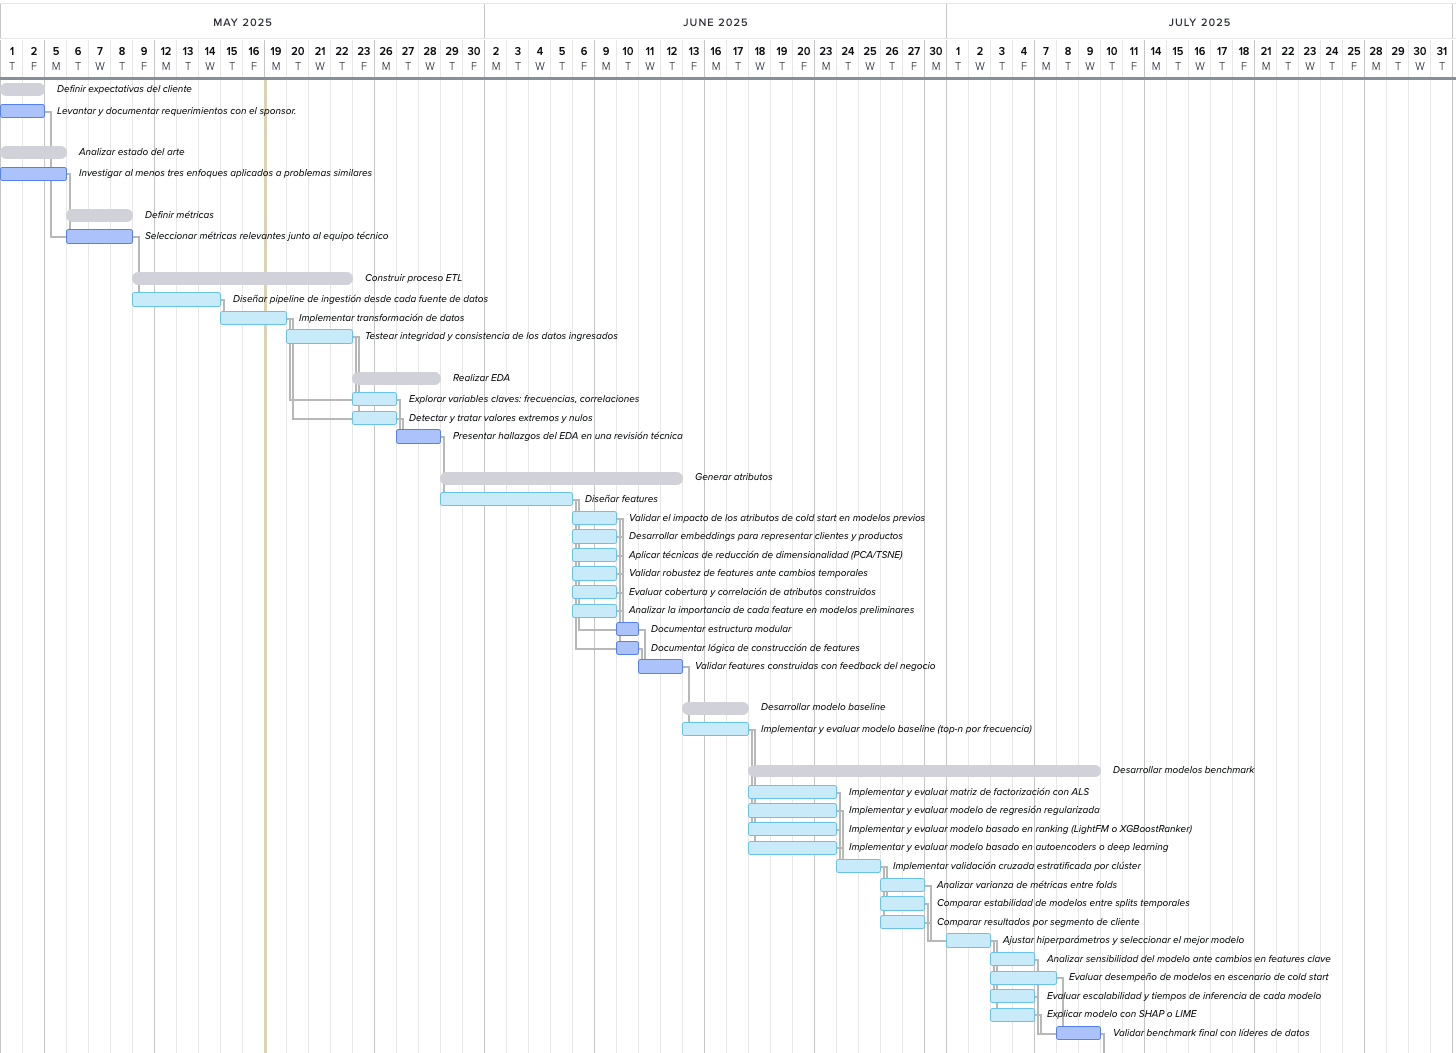
\includegraphics[width=.85\textwidth]{./Figuras/Gantt-1.png}
\caption{Diagrama de Gantt mayo a julio.}
\label{fig:diagBloques}
\end{figure}

\begin{figure}[htpb]
\centering 
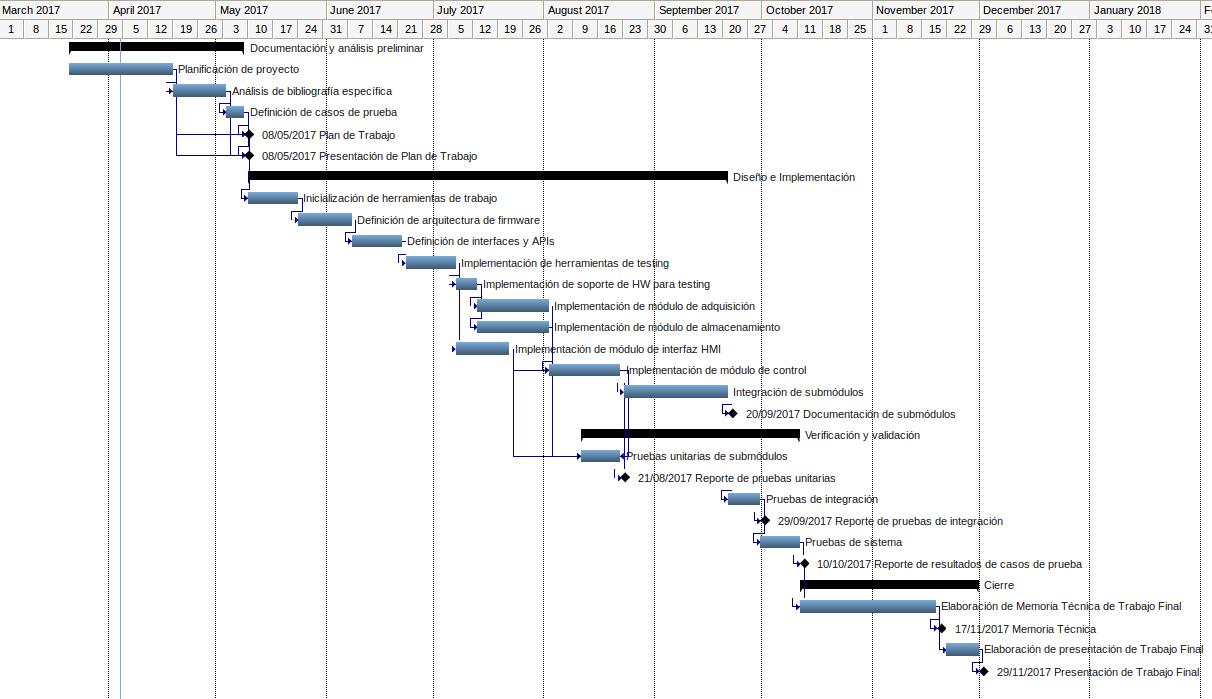
\includegraphics[width=.85\textwidth]{./Figuras/Gantt-2.png}
\caption{Diagrama de Gantt julio a septiembre.}
\label{fig:diagBloques}
\end{figure}


\begin{consigna}{red} % ELIMINAR \begin{consigna}{red} y \end{consigna}{red} en las secciones que vayan completando para cada entrega parcial.

El diagrama de Gantt debe representar de forma visual y cronológica todas las tareas del proyecto, abarcando aproximadamente 600 horas totales, de las cuales entre 480 y 500 deben destinarse a tareas técnicas (desarrollo, pruebas, implementación) y entre 100 y 120 a tareas no técnicas (planificación, documentación, escritura de memoria y preparación de la defensa).

\textbf{Consignas y recomendaciones:}
\begin{itemize}
  \item Incluir tanto tareas técnicas derivadas de las HU como tareas no técnicas generales del proyecto.
  \item El eje vertical debe listar las tareas y el eje horizontal representar el tiempo en semanas o fechas.
  \item Utilizar colores diferenciados para distinguir tareas técnicas y no técnicas.
  \item Las tareas deben estar ordenadas cronológicamente y reflejar todo el ciclo del proyecto.
  \item Iniciar con la planificación del proyecto (coincidente con el inicio de Gestión de Proyectos) y finalizar con la defensa, próxima a la fecha de cierre del trabajo.
  \item Configurar el software para mostrar los códigos del desglose de tareas y los nombres junto a cada barra.
  \item Asegurarse de que la fecha final coincida con la del Acta Constitutiva.
  \item Evitar tareas genéricas o ambiguas y asegurar una secuencia lógica y realista.
  \item Las fechas pueden ser aproximadas; ajustar el ancho del diagrama según el texto y el parámetro \texttt{x unit}. Para mejorar la apariencia del diagrama, es necesario ajustar este valor y, quizás, acortar los nombres de las tareas.
\end{itemize}

\textbf{Herramientas sugeridas:}
\begin{itemize}
  \item Planner, GanttProject, Trello + plugins\\
  \url{https://blog.trello.com/es/diagrama-de-gantt-de-un-proyecto}
  \item Creately (colaborativa online)\\
  \url{https://creately.com/diagram/example/ieb3p3ml/LaTeX}
  \item LaTeX con \texttt{pgfgantt}:\\
  \url{http://ctan.dcc.uchile.cl/graphics/pgf/contrib/pgfgantt/pgfgantt.pdf}
\end{itemize}

Incluir una imagen legible del diagrama de Gantt. Si es muy ancho, presentar primero la tabla y luego el gráfico de barras.

\begin{landscape}
\begin{figure}[htpb]
\centering 
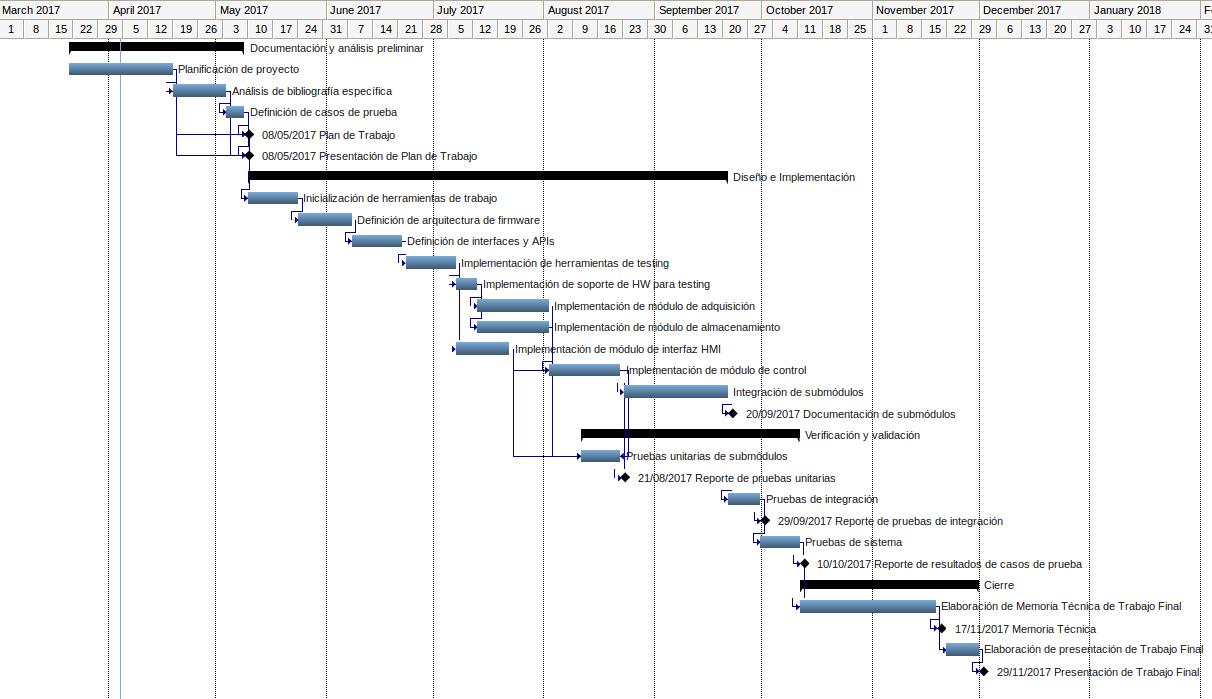
\includegraphics[height=.85\textheight]{./Figuras/Gantt-2.png}
\caption{Ejemplo de diagrama de Gantt (apaisado).} %Modificar este título acorde.
\label{fig:diagGantt}
\end{figure}

\end{landscape}

\end{consigna} % ELIMINAR \begin{consigna}{red} y \end{consigna}{red} en las secciones que vayan completando para cada entrega parcial.


\section{11. Planificación de Sprints}

\begin{consigna}{red} % ELIMINAR \begin{consigna}{red} y \end{consigna}{red} en las secciones que vayan completando para cada entrega parcial.

Organizar las tareas técnicas del proyecto en sprints de trabajo que permitan distribuir de forma equilibrada la carga horaria total, estimada en 600 horas.

\textbf{Consigna:}
\begin{itemize}
  \item Completar una tabla que relacione sprints con HU y tareas técnicas correspondientes.
  \item Incluir estimación en horas para cada tarea.
  \item Indicar responsable y porcentaje de avance estimado o completado.
  \item Contemplar también tareas de planificación, documentación, redacción de memoria y preparación de defensa.
\end{itemize}

\textbf{Conceptos clave:}
\begin{itemize}
  \item Una \'{e}pica es una unidad funcional amplia; una historia de usuario es una funcionalidad concreta; un sprint es una unidad de tiempo donde se ejecutan tareas.
  \item Las tareas son el nivel más desagregado: permiten estimar tiempos, asignar responsables y monitorear progreso.
\end{itemize}

\textbf{Duración sugerida:}
\begin{itemize}
  \item Para un proyecto de 600 h, se recomienda planificar entre 10 y 12 sprints de aproximadamente 2 semanas cada uno.
  \item Asignar entre 45 y 50 horas efectivas por sprint a tareas técnicas.
  \item Reservar 100 a 120 h para actividades no técnicas (planificación, escritura, reuniones, defensa).
\end{itemize}

\textbf{Importante:}
\begin{itemize}
  \item En proyectos individuales, el responsable suele ser el propio autor.
  \item Aun así, desagregar tareas facilita el seguimiento y mejora continua.
\end{itemize}

\textbf{Conversión opcional de Story Points a horas:}
\begin{itemize}
  \item 1 SP \(\approx\) 2 h como referencia flexible.
  \item Tener en cuenta aproximaciones tipo Fibonacci.
\end{itemize}

\begin{table}[htpb]
\centering
\caption{Formato sugerido}
\begin{tabularx}{\linewidth}{@{}|l|l|X|c|l|c|@{}}
\hline
\rowcolor[HTML]{C0C0C0}
Sprint & HU o fase & Tarea & Horas / SP & Responsable & \% Completado \\ \hline
Sprint 0 & Planificación & Definir alcance y cronograma & 10 h & Alumno & 100\% \\ \hline
Sprint 0 & Planificación & Reunión con tutor/cliente & 5 h & Alumno & 50\% \\ \hline
Sprint 0 & Planificación & Ajuste de entregables & 6 h & Alumno & 25\% \\ \hline
Sprint 1 & HU1 & Tarea 1 HU1 & 6 h / 3 SP & Alumno & 0\% \\ \hline
Sprint 1 & HU1 & Tarea 2 HU1 & 10 h / 5 SP & Alumno & 0\% \\ \hline
Sprint 2 & HU2 & Tarea 1 HU2 & 7 h / 5 SP & Alumno & 0\% \\ \hline
... & ... & ... & ... & ... & ... \\ \hline
Sprint 5 & Escritura & Redacción memoria & 50 h / 34 SP & Alumno & 0\% \\ \hline
Sprint 6 & Defensa & Preparación exposición & 20 h / 13 SP & Alumno & 0\% \\ \hline
\end{tabularx}
\end{table}

\textbf{Recomendaciones:}
\begin{itemize}
  \item Verificar que la carga horaria por sprint sea equilibrada.
  \item Usar sprints de 1 a 3 semanas, acordes al cronograma general.
  \item Actualizar el \% completado durante el seguimiento del proyecto.
  \item Considerar un sprint final exclusivo para pruebas, revisión y ajustes antes de la defensa.
\end{itemize}

\end{consigna} % ELIMINAR \begin{consigna}{red} y \end{consigna}{red} en las secciones que vayan completando para cada entrega parcial.


\section{12. Normativa y cumplimiento de datos (gobernanza)}

\begin{consigna}{red} % ELIMINAR \begin{consigna}{red} y \end{consigna}{red} en las secciones que vayan completando para cada entrega parcial.

En esta sección se debe analizar si los datos utilizados en el proyecto están sujetos a normativas de protección de datos y privacidad, y en qué condiciones se pueden emplear.

\textbf{Aspectos a considerar:}
\begin{itemize}
  \item Evaluar si los datos están regulados por normativas como GDPR, Ley 25.326 de Protección de Datos Personales en Argentina, HIPAA u otras según jurisdicción y temática.
  \item Determinar si el uso de los datos requiere consentimiento explícito de los usuarios involucrados.
  \item Indicar si existen restricciones legales, técnicas o contractuales sobre el uso, compartición o publicación de los datos.
  \item Aclarar si los datos provienen de fuentes licenciadas, de acceso público o bajo algún tipo de autorización especial.
  \item Analizar la viabilidad del proyecto desde el punto de vista legal y ético, considerando la gobernanza de los datos.
\end{itemize}

Este análisis es clave para garantizar el cumplimiento normativo y evitar conflictos legales durante el desarrollo y publicación del proyecto.

\end{consigna} % ELIMINAR \begin{consigna}{red} y \end{consigna}{red} en las secciones que vayan completando para cada entrega parcial.

\section{13. Gestión de riesgos}
\label{sec:riesgos}

\begin{consigna}{red} % ELIMINAR \begin{consigna}{red} y \end{consigna}{red} en las secciones que vayan completando para cada entrega parcial.
a) Identificación de los riesgos (al menos cinco) y estimación de sus consecuencias:
 
Riesgo 1: detallar el riesgo (riesgo es algo que si ocurre altera los planes previstos de forma negativa)
\begin{itemize}
	\item Severidad (S): mientras más severo, más alto es el número (usar números del 1 al 10).\\
	Justificar el motivo por el cual se asigna determinado número de severidad (S).
	\item Probabilidad de ocurrencia (O): mientras más probable, más alto es el número (usar del 1 al 10).\\
	Justificar el motivo por el cual se asigna determinado número de (O). 
\end{itemize}   

Riesgo 2:
\begin{itemize}
	\item Severidad (S): X.\\
	Justificación...
	\item Ocurrencia (O): Y.\\
	Justificación...
\end{itemize}

Riesgo 3:
\begin{itemize}
	\item Severidad (S):  X.\\
	Justificación...
	\item Ocurrencia (O): Y.\\
	Justificación...
\end{itemize}


b) Tabla de gestión de riesgos:      (El RPN se calcula como RPN=SxO)

\begin{table}[htpb]
\centering
\begin{tabularx}{\linewidth}{@{}|X|c|c|c|c|c|c|@{}}
\hline
\rowcolor[HTML]{C0C0C0} 
Riesgo & S & O & RPN & S* & O* & RPN* \\ \hline
       &   &   &     &    &    &      \\ \hline
       &   &   &     &    &    &      \\ \hline
       &   &   &     &    &    &      \\ \hline
       &   &   &     &    &    &      \\ \hline
       &   &   &     &    &    &      \\ \hline
\end{tabularx}%
\end{table}

Criterio adoptado: 

Se tomarán medidas de mitigación en los riesgos cuyos números de RPN sean mayores a...

Nota: los valores marcados con (*) en la tabla corresponden luego de haber aplicado la mitigación.

c) Plan de mitigación de los riesgos que originalmente excedían el RPN máximo establecido:
 
Riesgo 1: plan de mitigación (si por el RPN fuera necesario elaborar un plan de mitigación).
  Nueva asignación de S y O, con su respectiva justificación:
  \begin{itemize}
	\item Severidad (S*): mientras más severo, más alto es el número (usar números del 1 al 10).
          Justificar el motivo por el cual se asigna determinado número de severidad (S).
	\item Probabilidad de ocurrencia (O*): mientras más probable, más alto es el número (usar del 1 al 10).
          Justificar el motivo por el cual se asigna determinado número de (O).
	\end{itemize}

Riesgo 2: plan de mitigación (si por el RPN fuera necesario elaborar un plan de mitigación).
 
Riesgo 3: plan de mitigación (si por el RPN fuera necesario elaborar un plan de mitigación).

\end{consigna} % ELIMINAR \begin{consigna}{red} y \end{consigna}{red} en las secciones que vayan completando para cada entrega parcial.


\section{14. Sprint Review}
\label{sec:sprint_review}

\begin{consigna}{red} % ELIMINAR \begin{consigna}{red} y \end{consigna}{red} en las secciones que vayan completando para cada entrega parcial.

La revisión de sprint (\emph{Sprint Review}) es una práctica fundamental en metodologías ágiles. Consiste en revisar y evaluar lo que se ha completado al finalizar un sprint. En esta instancia, se presentan los avances y se verifica si las funcionalidades cumplen con los criterios de aceptación establecidos. También se identifican entregables parciales y se consideran ajustes si es necesario.

Aunque el proyecto aún se encuentre en etapa de planificación, esta sección permite proyectar cómo se evaluarán las funcionalidades más importantes del backlog. Esta mirada anticipada favorece la planificación enfocada en valor y permite reflexionar sobre posibles obstáculos.

\textbf{Objetivo:} anticipar cómo se evaluará el avance del proyecto a medida que se desarrollen las funcionalidades, utilizando como base al menos cuatro historias de usuario del \emph{Product Backlog}.


Seleccionar al menos 4 HU del Product Backlog. Para cada una, completar la siguiente tabla de revisión proyectada:

\textbf{Formato sugerido:}
\begin{table}[htpb]
\renewcommand{\arraystretch}{1.5}
\begin{tabular}{|>{\raggedright\arraybackslash}m{2.5cm}|
                >{\raggedright\arraybackslash}m{2.3cm}|
                >{\raggedright\arraybackslash}m{3cm}|
                >{\raggedright\arraybackslash}m{3cm}|
                >{\raggedright\arraybackslash}m{3cm}|}
\hline
\rowcolor[HTML]{CCCCCC}
\textbf{HU seleccionada} & \textbf{Tareas asociadas} & \textbf{Entregable esperado} & \textbf{¿Cómo sabrás que está cumplida?} & \textbf{Observaciones o riesgos} \\
\hline
                         & Tarea 1 &                             &                                           &                                     \\ \cline{2-2}
\multirow{-2}{=}{HU1}    & Tarea 2 & \multirow{-2}{=}{Módulo funcional} & \multirow{-2}{=}{Cumple criterios de aceptación definidos} & \multirow{-2}{=}{Falta validar con el tutor} \\
\hline
                         & Tarea 1 &                             &                                           &                                     \\ \cline{2-2}
\multirow{-2}{=}{HU3}    & Tarea 2 & \multirow{-2}{=}{Reporte generado} & \multirow{-2}{=}{Exportación disponible y clara} & \multirow{-2}{=}{Requiere datos reales} \\
\hline
                         & Tarea 1 &                             &                                           &                                     \\ \cline{2-2}
\multirow{-2}{=}{HU5}    & Tarea 2 & \multirow{-2}{=}{Panel de gestión} & \multirow{-2}{=}{Roles diferenciados operativos} & \multirow{-2}{=}{Riesgo en integración} \\
\hline
                         & Tarea 1 &                             &                                           &                                     \\ \cline{2-2}
\multirow{-2}{=}{HU7}    & Tarea 2 & \multirow{-2}{=}{Informe trimestral} & \multirow{-2}{=}{PDF con gráficos y evolución} & \multirow{-2}{=}{Puede faltar tiempo para ajustes} \\
\hline
\end{tabular}
\end{table}

\end{consigna} % ELIMINAR \begin{consigna}{red} y \end{consigna}{red} en las secciones que vayan completando para cada entrega parcial.


\section{15. Sprint Retrospective}    
\label{sec:sprint_retro}

\begin{consigna}{red} % ELIMINAR \begin{consigna}{red} y \end{consigna}{red} en las secciones que vayan completando para cada entrega parcial.

La retrospectiva de sprint es una práctica orientada a la mejora continua. Al finalizar un sprint, el equipo (o el alumno, si trabaja de forma individual) reflexiona sobre lo que funcionó bien, lo que puede mejorarse y qué acciones concretas pueden implementarse para trabajar mejor en el futuro.

Durante la cursada se propuso el uso de la \textbf{Estrella de la Retrospectiva}, que organiza la reflexión en torno a cinco ejes:

\begin{itemize}
\item  ¿Qué hacer más?
\item  ¿Qué hacer menos?
\item  ¿Qué mantener?
\item  ¿Qué empezar a hacer?
\item  ¿Qué dejar de hacer?
\end{itemize}

Aun en una etapa temprana, esta herramienta permite que el alumno planifique su forma de trabajar, identifique anticipadamente posibles dificultades y diseñe estrategias de organización personal.

\textbf{Objetivo:} reflexionar sobre las condiciones iniciales del proyecto, identificando fortalezas, posibles dificultades y estrategias de mejora, incluso antes del inicio del desarrollo.


Completar la siguiente tabla tomando como referencia los cinco ejes de la Estrella de la Retrospectiva (\emph{Starfish} o estrella de mar). Esta instancia te ayudará a definir buenas prácticas desde el inicio y prepararte para enfrentar el trabajo de forma organizada y flexible. Se deberá completar la tabla al menos para 3 sprints técnicos y 1 no técnico.

\textbf{Formato sugerido:}

\begin{table}[htpb]
\renewcommand{\arraystretch}{1.4}
\begin{tabular}{|>{\raggedright\arraybackslash}p{1.8cm}|
                >{\raggedright\arraybackslash}p{2.3cm}|
                >{\raggedright\arraybackslash}p{2.3cm}|
                >{\raggedright\arraybackslash}p{2.3cm}|
                >{\raggedright\arraybackslash}p{2.3cm}|
                >{\raggedright\arraybackslash}p{2.3cm}|}
\hline
\rowcolor[HTML]{CCCCCC} 
\textbf{Sprint tipo y N°} & \textbf{¿Qué hacer más?} & \textbf{¿Qué hacer menos?} & \textbf{¿Qué mantener?} & \textbf{¿Qué empezar a hacer?} & \textbf{¿Qué dejar de hacer?} \\
\hline
Sprint técnico - 1 & Validaciones continuas con el alumno & Cambios sin versión registrada & Pruebas con datos simulados & Documentar cambios propuestos & Ajustes sin análisis de impacto \\
\hline
Sprint técnico - 2 & Verificar configuraciones en múltiples escenarios & Modificar parámetros sin guardar historial & Perfiles reutilizables & Usar logs para configuración & Repetir pruebas manuales innecesarias \\
\hline
Sprint técnico - 8 & Comparar correlaciones con casos previos & Cambiar parámetros sin justificar & Revisión cruzada de métricas & Anotar configuraciones usadas & Trabajar sin respaldo de datos \\
\hline
Sprint no técnico - 12 (por ej.: ``Defensa'') & Ensayos orales con feedback & Cambiar contenidos en la memoria & Material visual claro & Dividir la presentación por bloques & Agregar gráficos difíciles de explicar \\
\hline
\end{tabular}
\end{table}

\end{consigna} % ELIMINAR \begin{consigna}{red} y \end{consigna}{red} en las secciones que vayan completando para cada entrega parcial.

\end{document}